\documentclass[12pt, a4paper]{article}
\usepackage[utf8]{inputenc}
\usepackage{mathtools}
\usepackage{amsthm}
\usepackage{cancel}

\usepackage{esint}

\usepackage{graphicx}
\graphicspath{ {../images/} }

\usepackage{listings}
\usepackage{xcolor}

\usepackage[T1]{fontenc}

\definecolor{codegreen}{rgb}{0,0.6,0}
\definecolor{codegray}{rgb}{0.5,0.5,0.5}
\definecolor{codepurple}{rgb}{0.58,0,0.82}
\definecolor{backcolour}{rgb}{0.95,0.95,0.92}

\lstdefinestyle{mystyle}{
    backgroundcolor=\color{backcolour},   
    commentstyle=\color{codegreen},
    keywordstyle=\color{blue},
    numberstyle=\tiny\color{codegray},
    stringstyle=\color{codegreen},
    basicstyle=\ttfamily\footnotesize,
    breakatwhitespace=false,         
    breaklines=true,                 
    captionpos=b,                    
    keepspaces=true,                 
    numbers=left,                    
    numbersep=5pt,                  
    showspaces=false,                
    showstringspaces=false,
    showtabs=false,                  
    tabsize=2
}

\lstset{style=mystyle}

\title{Obligatorisk oppgave 1, MEK1100, Vår 2021}
\author{Cory Alexander Balaton}
\date{}

\begin{document}

\maketitle 
\newpage


\section*{Oppgave 1}
\begin{equation*}
    \begin{split}
        x(t) &= v_0 \cdot t \cdot \cos(\theta) \\
        y(t) &= v_0 \cdot t \cdot \sin(\theta) - \frac{1}{2} \cdot g \cdot t^2 
    \end{split}
\end{equation*} \\
a) \\
For å finne $t_m$, så må vi finne nullpunktene til $y(t)$:
\begin{equation}
    \begin{split}
                                                                  y(t) &= 0 \\
        v_0 \cdot t \cdot \sin(\theta) - \frac{1}{2} \cdot g \cdot t^2 &= 0 \\
        t \cdot (v_0 \cdot \sin(\theta) - \frac{1}{2} \cdot g \cdot t) &= 0 \\
    \end{split}
\end{equation}
\begin{equation}
    \begin{split}
        t_0 = 0
    \end{split}
\end{equation}
\begin{equation}
    \begin{split}
        v_0 \cdot \sin(\theta) - \frac{1}{2} \cdot g \cdot t_m &= 0 \\
                                      v_0 \cdot \sin(\theta) &= \frac{1}{2} \cdot g \cdot t_m \\
                                                         t_m &= \frac{2 \cdot v_0 \cdot \sin(\theta)}{g}
    \end{split}
\end{equation}
\begin{equation}
    \begin{split}
        x_m &= x(t_m) \\
            &= v_0 \cdot \frac{2 \cdot v_0 \cdot \sin(\theta)}{g} \cdot \cos(\theta) \\
            &= \frac{2 \cdot v_0^2 \cdot \sin(\theta) \cdot \cos(\theta)}{g}
    \end{split}
\end{equation}

\newpage
\section*{Oppgave 2}

\begin{equation}
    \textbf{v} = (x \cdot y, y)
\end{equation}
\\
a) \\
For å finne strømningslinjene, så må vi sette opp likningen:

\begin{equation}
    \begin{split}
        \frac{dy}{dx} &= \frac{y}{x \cdot y} \\
                   dy &= \frac{1}{x} dx \\
                    y &= \ln|x| + c
    \end{split}
\end{equation}
\\
b) \\ \\
\hspace*{-1.5cm}
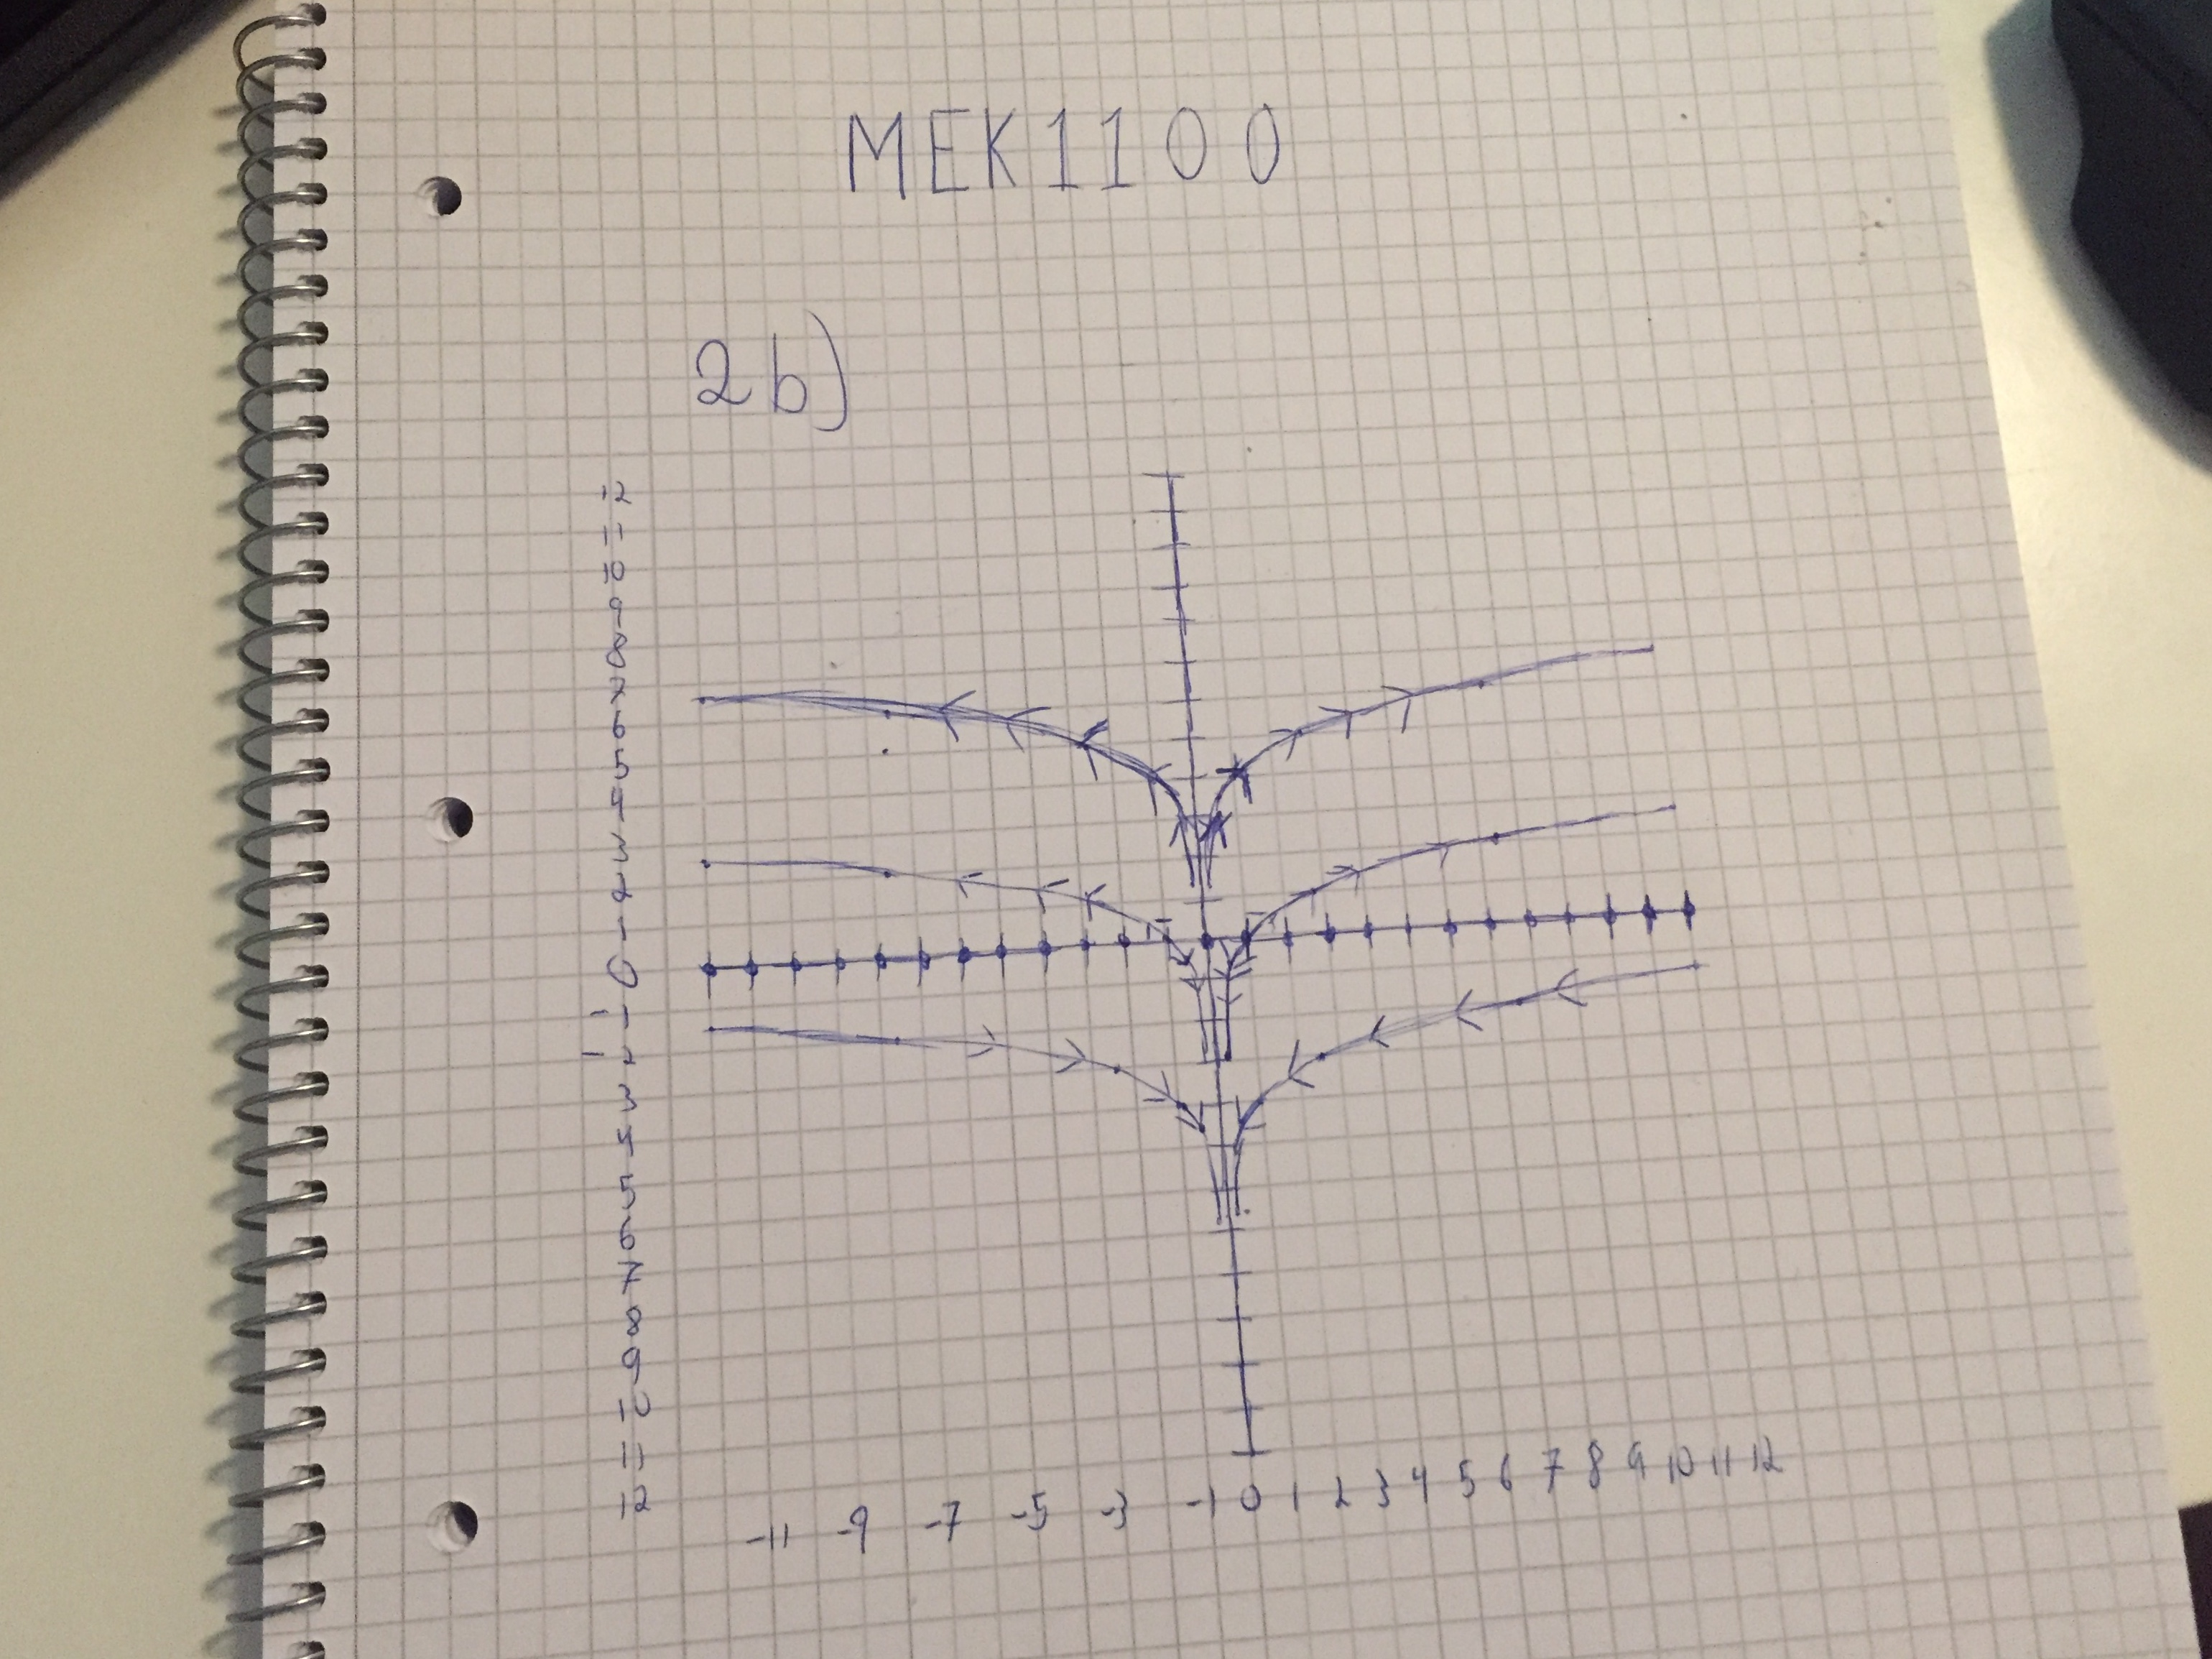
\includegraphics[scale=0.15]{two_b_hand_drawn}


\newpage
Python program:
\lstinputlisting[language=Python]{../Python/two_b.py}

\newpage
Output: \\
\hspace*{-1.5cm}
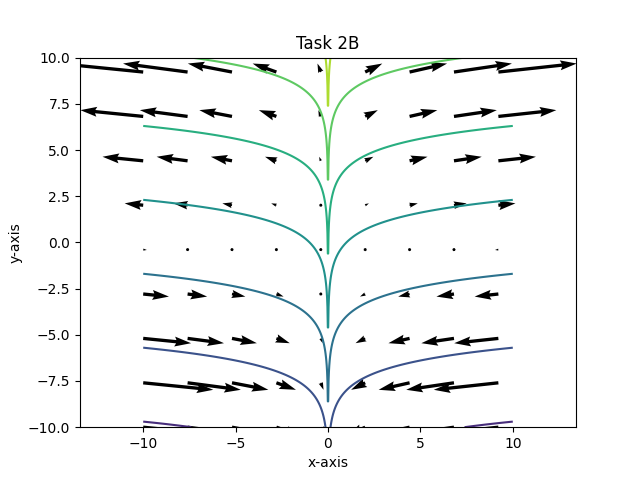
\includegraphics{two_b}
\\
c) \\
Hvis en strømfunksjon eksisterer, så må vektorfeltet være divergensfritt.

\begin{equation}
    \begin{split}
        \nabla \cdot \textbf{v} &= \frac{\partial v_x}{\partial x} + \frac{\partial v_y}{\partial y} \\
                                &= \frac{\partial}{\partial x} x \cdot y + \frac{\partial}{\partial y} y \\
                                &= y + 1 \\
                                &\neq 0
    \end{split}
\end{equation}

Siden divergensen til $v$ ikke er $0$, så eksisterer det ingen strømfunksjon.




\newpage
\section*{Oppgave 3}

\begin{equation}
    \textbf{v} = (\cos(x) \cdot \sin(y), -\sin(x) \cdot \cos(y))
\end{equation}
\\
a)\\
Divergensen blir lik:

\begin{equation}
    \begin{split}
        \nabla \cdot \textbf{v} &= \frac{\partial v_x}{\partial x} + \frac{\partial v_y}{\partial y} \\
                                &= \frac{\partial}{\partial x} \cos(x) \cdot \sin(y) + \frac{\partial}{\partial y} -\sin(x) \cdot \cos(y) \\
                                &= -\sin(x) \cdot \sin(y) + \sin(x) \cdot \sin(y) \\
                                &= 0
    \end{split}
\end{equation}
\\
Virvlingen blir lik:

\begin{equation}
    \begin{split}
        \nabla \times \textbf{v} &= (\frac{\partial v_y}{\partial x} - \frac{\partial v_x}{\partial y}) \cdot \textbf{k} \\
                                 &= (\frac{\partial}{\partial x} -\sin(x) \cdot \cos(y) - \frac{\partial}{\partial y} \cos(x) \cdot \sin(y)) \cdot \textbf{k} \\
                                 &= (-\cos(x) \cdot \cos(y) - cos(x) \cdot \cos(y)) \cdot \textbf{k} \\
                                 &= (-2 \cdot cos(x) \cdot \cos(y)) \cdot \textbf{k}
    \end{split}
\end{equation}
\\
b) \\
Python kode: \\
\lstinputlisting[language=Python]{../Python/three_b.py}
Feltet som blir produsert: \\
\hspace*{-1.5cm}
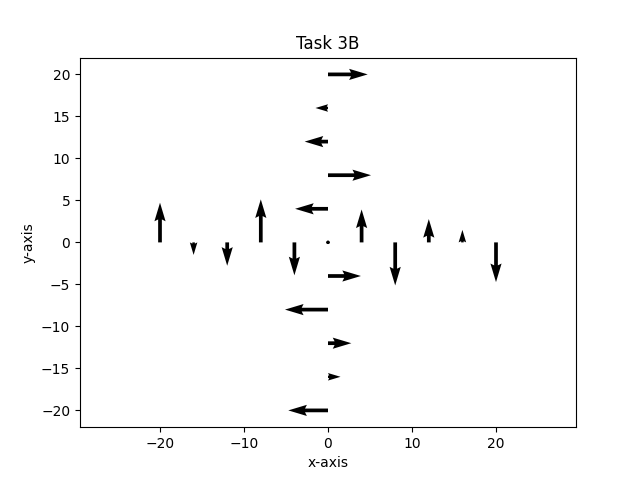
\includegraphics[scale=0.8]{three_b}

c) \\
\begin{equation}
    \textbf{F} = \textbf{v}
\end{equation}
Man kan først definere randa til kvadratet med $4$ parametere:
\begin{equation}
    \begin{split}
        \textbf{r}_1(t) &= \left(\frac{\pi}{2}, t \right) \\
        \textbf{r}_2(t) &= \left(-\frac{\pi}{2}, t \right) \\
        \textbf{r}_3(t) &= \left(t, \frac{\pi}{2} \right) \\
        \textbf{r}_4(t) &= \left(t, -\frac{\pi}{2} \right) \\
    \end{split}
\end{equation}
Deretter tar man linjeintegralet til $\textbf{F}$ med hver parameter og adderer dem sammen: \\
\begin{equation}
    \begin{split}
        \ointctrclockwise_C &= \int_{-\frac{\pi}{2}}^{\frac{\pi}{2}} \textbf{F}(\textbf{r}_1(t)) \cdot \textbf{r}_1'(t) \cdot j \; dt \\
                        &+ \int_{-\frac{\pi}{2}}^{\frac{\pi}{2}} \textbf{F}(\textbf{r}_2(t)) \cdot \textbf{r}_2'(t) \cdot -j \; dt \\
                        &+ \int_{-\frac{\pi}{2}}^{\frac{\pi}{2}} \textbf{F}(\textbf{r}_3(t)) \cdot \textbf{r}_3'(t) \cdot -i \; dt \\
                        &+ \int_{-\frac{\pi}{2}}^{\frac{\pi}{2}} \textbf{F}(\textbf{r}_4(t)) \cdot \textbf{r}_4'(t) \cdot i \; dt \\
    \end{split}
\end{equation} \\
\begin{equation}
    \begin{split}
        \int_{-\frac{\pi}{2}}^{\frac{\pi}{2}} \textbf{F}(\textbf{r}_1(t)) \cdot \textbf{r}_1'(t) \cdot j \; dt &= \int_{-\frac{\pi}{2}}^{\frac{\pi}{2}} (\cos\left(\frac{\pi}{2}\right)\sin(t) \cdot i - \sin\left(\frac{\pi}{2}\right)\cos(t) \cdot j) \cdot j \; dt \\
        &= \int_{-\frac{\pi}{2}}^{\frac{\pi}{2}} (- \cos(t) \cdot j) \cdot j \; dt \\
        &= \left[- \sin(t) \right]_{-\frac{\pi}{2}}^{\frac{\pi}{2}} \\
        &= - 1 - 1 \\
        &= -2
    \end{split}
\end{equation}
\begin{equation}
    \begin{split}
        \int_{-\frac{\pi}{2}}^{\frac{\pi}{2}} \textbf{F}(\textbf{r}_2(t)) \cdot \textbf{r}_2'(t) \cdot (-j) \; dt &= \int_{-\frac{\pi}{2}}^{\frac{\pi}{2}} (\cos(-\frac{\pi}{2})\sin(t) \cdot i - \sin(-\frac{\pi}{2})\cos(t) \cdot j) \cdot (-j) \; dt \\
        &= \int_{-\frac{\pi}{2}}^{\frac{\pi}{2}} (\cos(t) \cdot j) \cdot (-j) \; dt \\
        &= \left[- \sin(t) \right]_{-\frac{\pi}{2}}^{\frac{\pi}{2}} \\
        &= - 1 - 1 \\
        &= -2
    \end{split}
\end{equation}
\begin{equation}
    \begin{split}
        \int_{-\frac{\pi}{2}}^{\frac{\pi}{2}} \textbf{F}(\textbf{r}_3(t)) \cdot \textbf{r}_3'(t) \cdot (-i) \; dt &= \int_{-\frac{\pi}{2}}^{\frac{\pi}{2}} (\cos(t)\sin\left(\frac{\pi}{2}\right) \cdot i - \sin(t)\cos\left(\frac{\pi}{2}\right) \cdot j) \cdot (-i) \; dt \\
        &= \int_{-\frac{\pi}{2}}^{\frac{\pi}{2}} (\cos(t) \cdot i) \cdot (-i) \; dt \\
        &= \left[- \sin(t) \right]_{-\frac{\pi}{2}}^{\frac{\pi}{2}} \\
        &= - 1 - 1 \\
        &= -2
    \end{split}
\end{equation}
\begin{equation}
    \begin{split}
        \int_{-\frac{\pi}{2}}^{\frac{\pi}{2}} \textbf{F}(\textbf{r}_4(t)) \cdot \textbf{r}_4'(t) \cdot i \; dt &= \int_{-\frac{\pi}{2}}^{\frac{\pi}{2}} (\cos(t)\sin\left(-\frac{\pi}{2}\right) \cdot i - \sin(t)\cos\left(-\frac{\pi}{2}\right) \cdot j) \cdot i \; dt \\
        &= \int_{-\frac{\pi}{2}}^{\frac{\pi}{2}} (- \cos(t) \cdot i) \cdot i \; dt \\
        &= \left[- \sin(t) \right]_{-\frac{\pi}{2}}^{\frac{\pi}{2}} \\
        &= - 1 - 1 \\
        &= -2
    \end{split}
\end{equation}
Sirkulasjonen blir da:
\begin{equation}
    \ointctrclockwise_C = -2 + (-2) + (-2) + (2) = -8
\end{equation}
\\
d) \\
Siden $\nabla \cdot \textbf{v} = 0$, så betyr det at feltet er konservativt og derfor finnes det en strømfunksjon for feltet. \\
For å regne ut $\psi$, så må man først finne $\int \frac{\partial \psi}{\partial x}$ og $\int \frac{\partial \psi}{\partial y}$

\begin{equation}
    \begin{split}
        \int \frac{\partial \psi}{\partial y} &= \int v_x dy \\
                                              &= \int \cos(x) \cdot \sin(y) dx \\
                                              &= \cos(x) \cdot \cos(y) + f(x)
    \end{split}
\end{equation}

\begin{equation}
    \begin{split}
        \int \frac{\partial \psi}{\partial x} &= \int v_y dx \\
                                              &= \int -\sin(x) \cdot \cos(y) dx \\
                                              &= \cos(x) \cdot \cos(y) + g(y)
    \end{split}
\end{equation}

Ut i fra det vi har regnet ut, så ser vi at strømningsfunksjonen blir $\psi = \cos(x) \cdot \cos(y)$.



\newpage
\section*{Oppgave 4}

a)
\lstinputlisting[language=Python]{../Python/strlin.py}
Koden over gir to plotter: \\
\hspace*{-1.5cm}
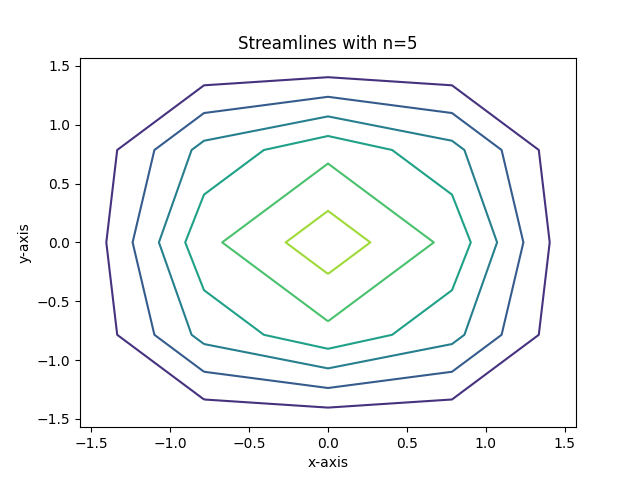
\includegraphics[scale=0.5]{strlin_5}
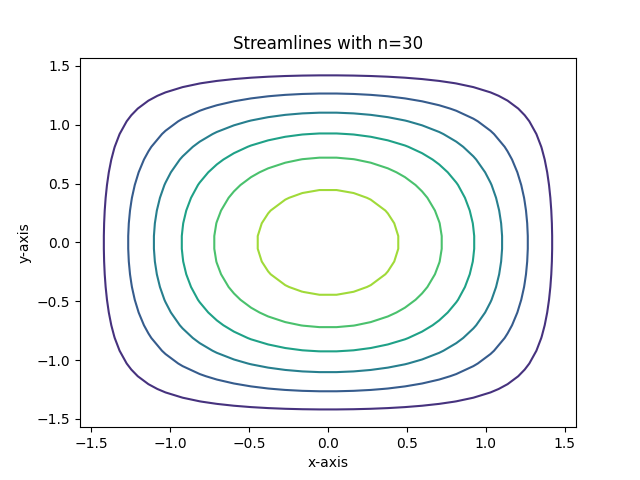
\includegraphics[scale=0.5]{strlin_30}\\

b)
\lstinputlisting[language=Python]{../Python/vec.py}
Koden over gir vektorfeltet under: \\
\hspace*{-1.5cm}
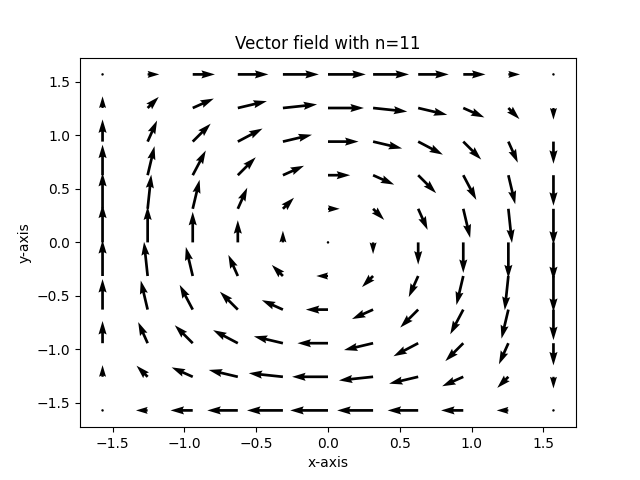
\includegraphics[scale=1]{vec_11.png}


\end{document}